% !TEX root = ../Thesis.tex
\chapter{Sudoku Variants and Rules}\label{SudokuVariantsAndRules}
This chapter introduces the most common Sudoku variants and rules used in CTCGH \cite{CrackingTheCryptic2021}, which are all based on the normal Sudoku rules introduced in Section \ref{NormalSudoku}. Meaning the normal Sudoku rules still apply, in addition to the rules of the variants introduced in this chapter. The aim here is to give an overview, so the descriptions are on a high level and relatively informal. All A formal definition and further details on how the constraints and types are encoded to CNF can be found in chapter \ref{Encoding}.

\section{Killer Sudoku}
In a Killer Sudoku, the normal Sudoku rules apply. Additionally, some (not necessarily all) orthogonally adjacent cells are grouped in so-called cages. Each cell can be part of at most one cage. For each cage, two constraints must hold, firstly, the values of all its cells must have a certain sum (\emph{target sum}), and within a cage, each value may only appear once. The cages are often marked on the grid with dashed lines or by colouring their cells, and a small number is placed in the top-left cell of a cage to specify its targeted sum. See Figure \ref{fig:exampleKiller} for an example.

\begin{figure}
\centering
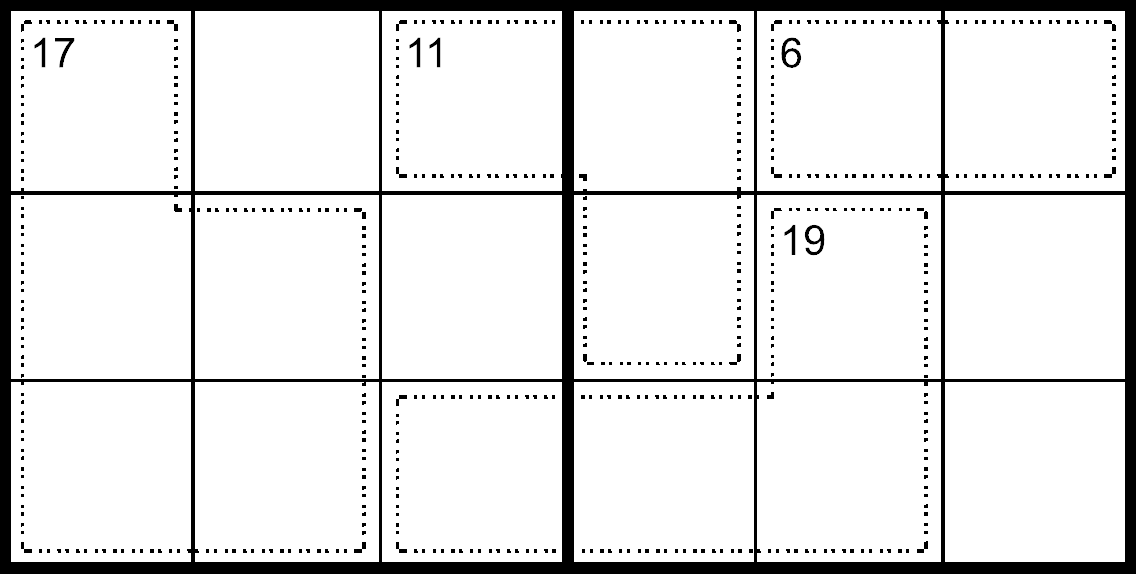
\includegraphics[width=0.6\textwidth]{Figures/Killer Example (CTC page 36).png}
\caption{Section of a Killer Sudoku showing 4 cages, from CTCGH \cite{CrackingTheCryptic2021} page 36.}
\label{fig:exampleKiller}
\end{figure}

\section{Thermometers}
Thermometers placed on the Sudoku grid connect multiple adjacent cells sequentially (without branching). Each thermometer has a bulb cell marked with a filled circle, and its other cells are marked with a line outgoing from this circle. For a thermometer, it must hold that starting from the bulb, the cell values along the thermometer can only strictly increase. CTCGH \cite{CrackingTheCryptic2021} also contains a version called ``Frozen Thermometers" that allows cell values along a thermometer to stay the same. Additionally, it differs from puzzle to puzzle instance, whether thermometers are allowed to overlap each other or not.

Thermometers are also part of the unique puzzle on page 52 of CTCGH \cite{CrackingTheCryptic2021}. In this puzzle, only three hint digits and the shape and orientation of 8 thermometers are given. It is then up to the solver to deduce the position of the thermometers, which can not overlap.\todoMissing{Figure}

\section{Sandwich Sums}
Sandwich Sums are constraints that can be applied to rows, columns or cages. They require certain cells to have a particular sum, which is specified for each row and column at the grid's edge or inside an affected cage. To fulfill a Sandwich Sum Constraint, it must hold that the sum of all cells lying between the cells containing the values 1 and 9 is equal to the specified target sum. The cells containing 1 and 9 are not included in the sum. Example: a row containing the numbers [2, 4, 8, 9, 6, 5, 1, 7, 9] has a Sandwich Sum of 6 + 5 = 11. CTCGH \cite{CrackingTheCryptic2021} also includes a variation ``Sandwich Sums - 1 to X", where a target sum must be hit, but the second value that defines the sums border is not defined and must be deduced to a value of 2 to 9.\todoMissing{Figure}

\section{Secret Direction}
The Secret Direction constraints is used in a unique Sudoku Puzzle described on page 41 of CTCGH \cite{CrackingTheCryptic2021}. Following an adventure's backstory to find a buried treasure, the constraint requires a solution with a ``secret path" from a shaded starting cell to the only cell with value 9, which is also the centre of a 3x3 box. The hidden path must be reconstructed in the following way, starting with the shaded cell; the current cell's value describes the length of the next step, and the position of the 9 in the current 3x3 box defines the direction. Once a step in the path is found, one must apply the same rules to find the next one until the treasure is discovered.

\section{Arrowheads}
Arrowheads placed on the Sudoku grid specify the partial or total order that must be respected between two adjacent cell values.

\section{Chess Moves}
Some Sudoku Variants use constraints named after chess figures to describe the relationship between two different cells. In CTCGH \cite{CrackingTheCryptic2021}, three of these constraints are introduced, which share the idea that if another cell can be reached from a cell by one chess move of a particular chess figure, these cells may not have the same value. The three constraints differ in the chess figure they use, as listed below.
\begin{itemize}
    \item Anti-Knight: Cells that are one knight move away from each other may not contain the same value. A knight move consists either of one or two steps in one direction on the current column or row followed by either one or two steps in the then-current row or column. In total, the length must be three steps, and a column and row must be used.
    \item Anti-King: Cells that are one king move away from each other may not contain the same value. The set of cells that are one king move away from a cell is equal to the set of cells that are directly orthogonally and diagonally adjacent to it.
    \item Anti-Queen: Cells that are one queen move away from each other may not contain the same value. Cells that are one queen move away from a cell are the cells that lie on the same row, column or diagonal as a cell.
\end{itemize}

\section{Towers}
The name Towers is used for a unique constraint in the puzzle on page 49 of CTCGH \cite{CrackingTheCryptic2021}. A tower describes a group of cells which is always based at the lowest row (nr. 9) and rises to a certain height. The different towers are marked by the differently shaded cells. Furthermore, below each tower at the grid's edge stands a number representing its target sum. There are two types of towers, normal and faulty ones. In a normal tower, the cell values are strictly increasing starting from the base and adding all its cell values together results in the target sum. Differently, the numbers are not strictly increasing, or the sums do not match in a faulty tower, but not both at once. As an additional help, it is stated how many towers have non-increasing values and for how many towers the sums will not match. However, it is then up to the solver to deduce which towers belong to which type.
\todoMissing{Nurikabe Sudoku}